\chapter{Discusión de Resultados}
% \blindtext

En este capítulo intentaremos dar respuesta a las preguntas planteadas en la introducción con base a lo visto en los capítulos anteriores.

\subsection*{¿Existe una diferencia en el desempeño del algoritmo PFI-EMOA al variar la combinación los pesos?}

Claramente si existe una diferencia, como podemos ver en las Figuras \ref{fig:KW_dim_IGDp}, \ref{fig:KW_dim_R2}, \ref{fig:KW_conv_dist_IGDp} y \ref{fig:KW_conv_dist_R2}, . También notamos en estas Figuras que la elección del indicador de convergencia del algoritmo PFI-EMOA importa mucho para la sensibilidad con respecto a la combinación de pesos. En particular, R2 es mucho menos sensible que IGD+. Este resultado es importante ya que PFI-EMOA demostró ser mejor que muchos MOEAs  y en este trabajo hemos mostrado que la elección de los pesos en la escalarización de Tchebycheff sí importa. Sobre todo metiéndonos más en detalles acerca de la aproximación final, es decir, si el DM quisiera una solución con mayor SPD sabríamos que tenemos que una buena heurística sería darle mayor peso a los primero valores. 

\subsection*{¿Qué combinación de pesos es mejor para cada problema?}

Usando las agregaciones mostradas en el capítulo anterior en las Figuras \ref{fig:borda_obj_2}, \ref{fig:borda_obj_3}, \ref{fig:borda_obj_4}, \ref{fig:borda_obj_5}, \ref{fig:borda_obj_6} y \ref{fig:borda_obj_7} podemos tener una idea que el número de objetivos del problema si afecta a la elección de pesos. En particular el hecho de que para dos dimensiones parezca no importar indica que tal vez los objetivos de ambos indicadores están alineados hasta cierto punto y parece suceder lo mismo cuando los objetivos se vuelven mayores que 5. Agrupando sobre la categoría de los indicadores notamos de las Figuras \ref{fig:borda_hv}, \ref{fig:borda_epsp}, \ref{fig:borda_R2}, \ref{fig:borda_igd} y \ref{fig:borda_igdp}  que los indicadores de convergencia que son consistentes de Pareto si crecen conforme le damos más importancia a IGD+, teniendo nuevamente resultados aparentemente sin patrones tan claros cuando usamos R2 en el estimador de densidad. Mientras que los indicadores de diversidad que se muestran en la Figura \ref{fig:borda_senergy}, \ref{fig:borda_spd} tienen comportamientos opuestos. El caso más interesante tal vez sea el de Energía-S que empeora su desempeño mientras lo priorizamos más (aumentando $w_0$), de esta manera parecería que si se quiere obtener una solución con mayor Energía-S no se tiene que buscar optimizar este indicador en cada paso.   

Nuevamente no encontramos ningún comportamiento notorio en los resultados del algoritmo que usa a R2. Es importante notar que no necesariamente se le da más importancia a uno u a otro indicador siempre. Sino que, como se explica en la Sección \ref{sec:PFI-EMOA}, el algoritmo entra a la parte del estimador de densidad cuando no encuentra más de una solución que contribuye lo mismo para cambiar el indicador de IGD+ (como se puede ver en la línea 6 de el Algoritmo \ref{alg:PFI-EMOA}). Entonces, el efecto que tengan los diferentes pesos también se verá afectado con cuántas veces sea esta situación relevante. Así, podría pasar que es importante para algún algoritmo priorizar más un indicador, sin embargo, no se le da la oportunidad de tener un efecto tan grande.  


\subsection*{¿Qué sucede cuando cambiamos el indicador de convergencia de IGD$+$ a R2?}

Aunque ya hemos visto que hay menos sensibilidad a los pesos por parte del indicador R2, en esta sección miraremos esto con mayor detalle, haciendo las comparaciones de algoritmos directamente entre IGD+ y R2. Por ejemplo, para hacer el análisis de las Figuras \ref{fig:R2_vs_IGDp_2}, \ref{fig:R2_vs_IGDp_3}, \ref{fig:R2_vs_IGDp_4}, \ref{fig:R2_vs_IGDp_5}, \ref{fig:R2_vs_IGDp_6} y \ref{fig:R2_vs_IGDp_7}, para cada configuración de pesos, se tomaron los algoritmos de IGD+ y R2 y se compararon usando Wilcoxon, así se promediaron 11 comparaciones para ver en cuál ganaba cierto algoritmo. Cabe destacar que para este caso se tuvo que cambiar el signo de los indicadores que se tienen que minimizar para poder usar la prueba de Wilcoxon y ver si el algoritmo de IGD+ era mayor al algoritmo de R2 o viceversa.


\begin{figure} [H]
    \centering
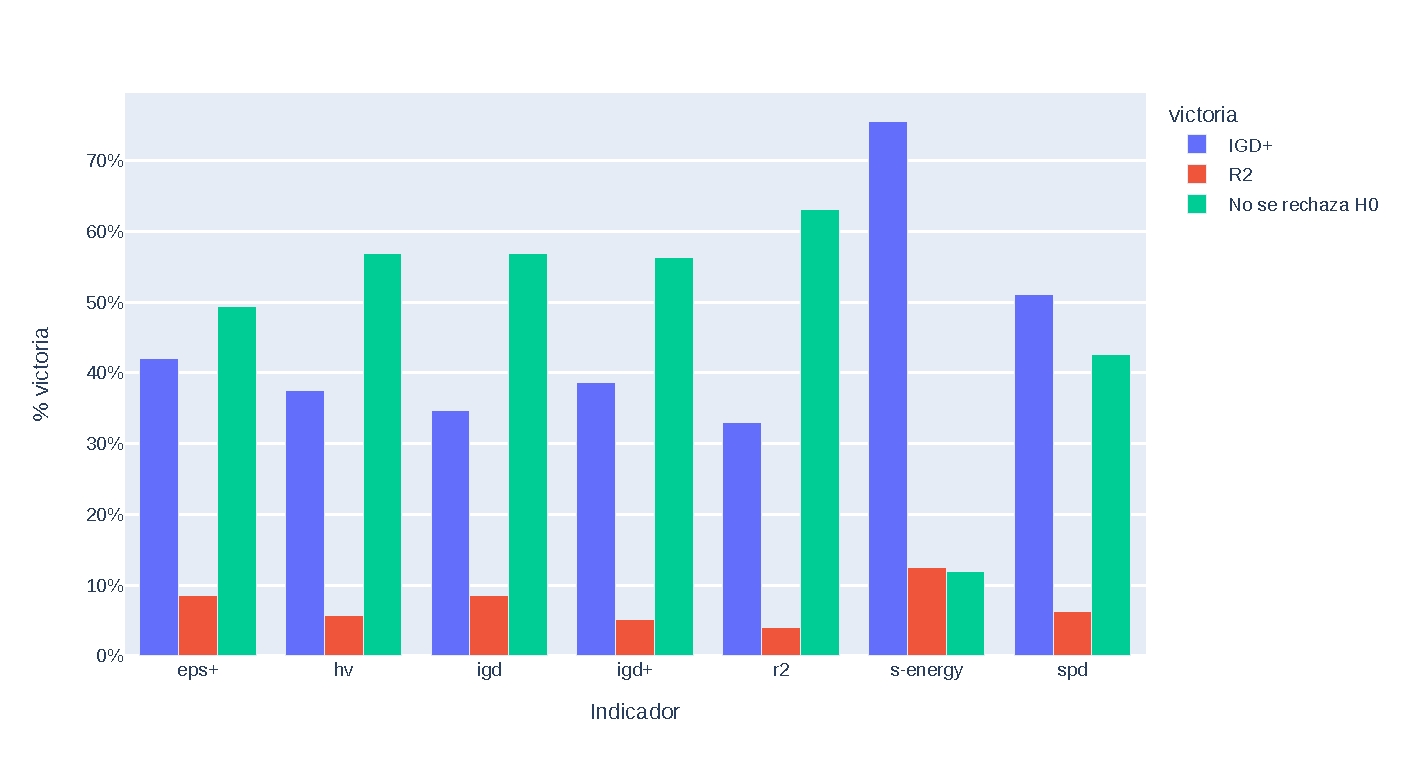
\includegraphics[width=\textwidth]{Figuras/R2_vs_IGDp_nobj2.pdf}
\caption[IGD+ vs R2 2 objetivos]{Porcentaje de victorias de diferentes indicadores de convergencia en la esclarización de Tchebycheff para 2 objetivos.}
\label{fig:R2_vs_IGDp_2}
\end{figure}

\begin{figure} [H]
    \centering
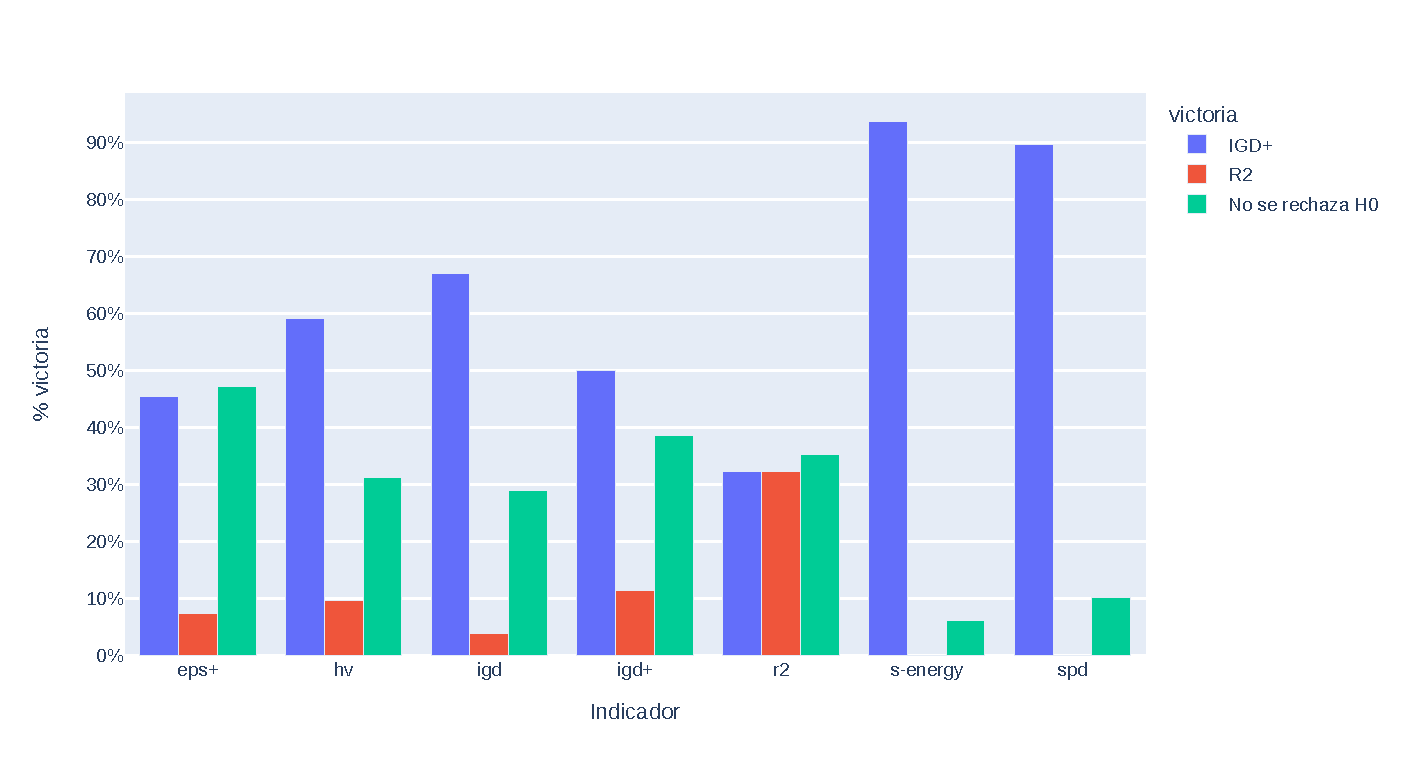
\includegraphics[width=\textwidth]{Figuras/R2_vs_IGDp_nobj3.pdf}
\caption[IGD+ vs R2 3 objetivos]{Porcentaje de victorias de diferentes indicadores de convergencia en la esclarización de Tchebycheff para 3 objetivos.}
\label{fig:R2_vs_IGDp_3}
\end{figure}

\begin{figure} [H]
    \centering
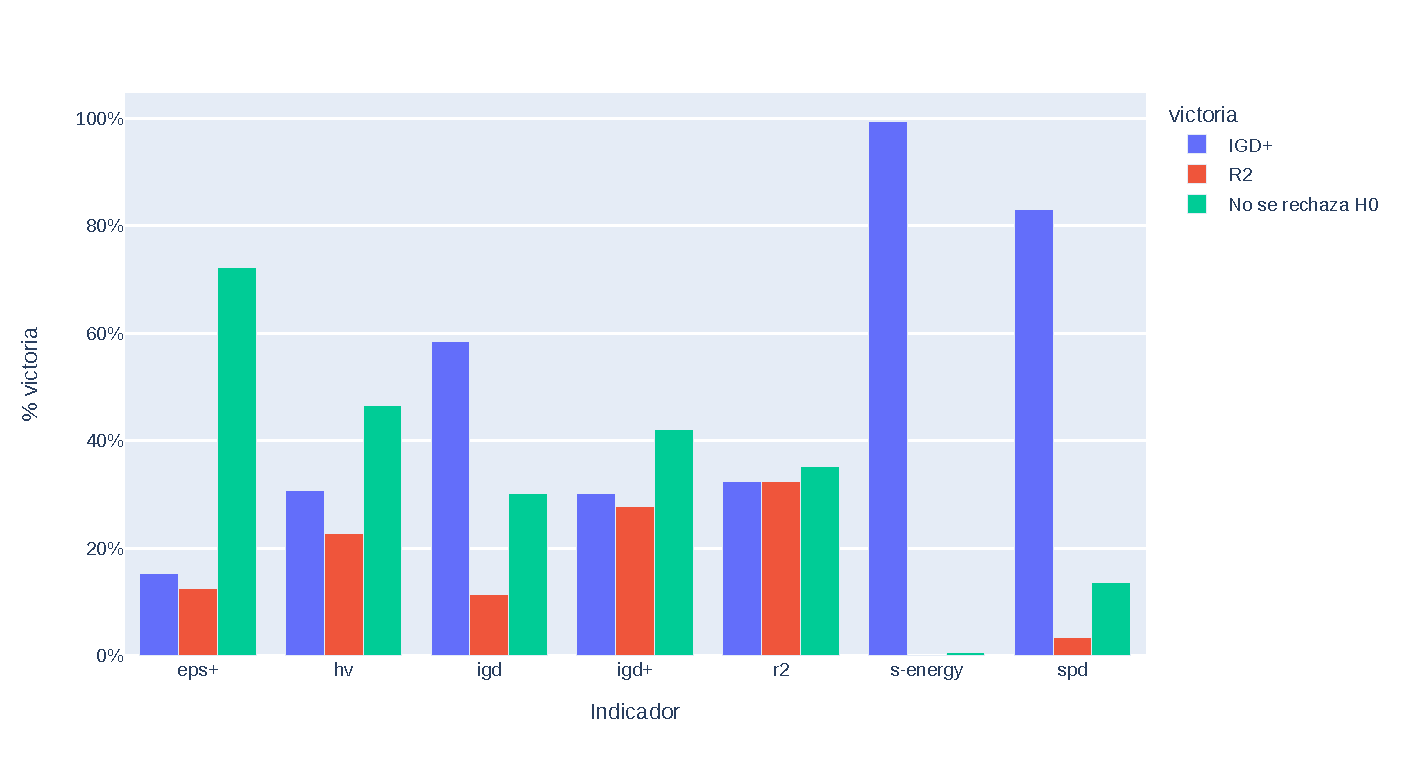
\includegraphics[width=\textwidth]{Figuras/R2_vs_IGDp_nobj4.pdf}
\caption[IGD+ vs R2 4 objetivos]{Porcentaje de victorias de diferentes indicadores de convergencia en la esclarización de Tchebycheff para 4 objetivos.}
\label{fig:R2_vs_IGDp_4}
\end{figure}

\begin{figure} [H]
    \centering
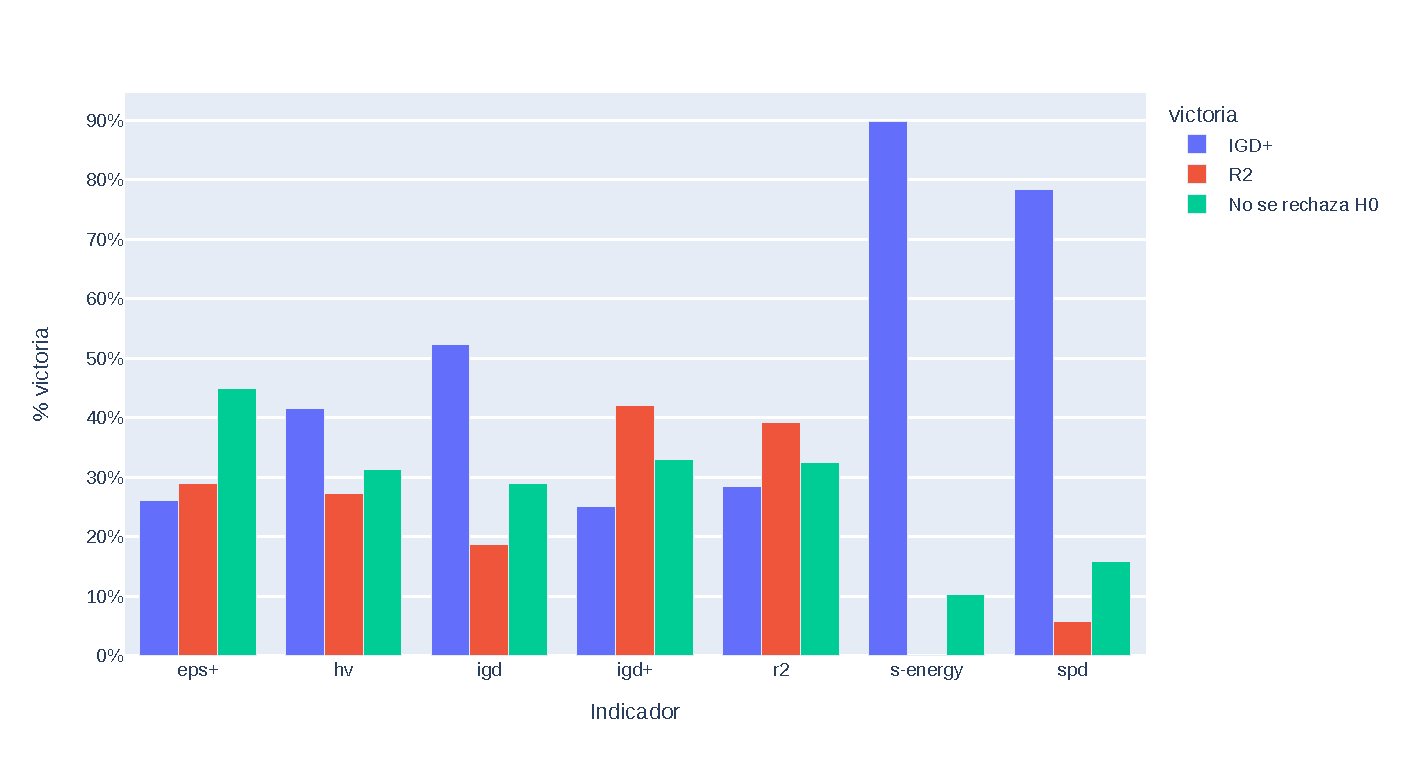
\includegraphics[width=\textwidth]{Figuras/R2_vs_IGDp_nobj5.pdf}
\caption[IGD+ vs R2 5 objetivos]{Porcentaje de victorias de diferentes indicadores de convergencia en la esclarización de Tchebycheff para 5 objetivos.}
\label{fig:R2_vs_IGDp_5}
\end{figure}

\begin{figure} [H]
    \centering
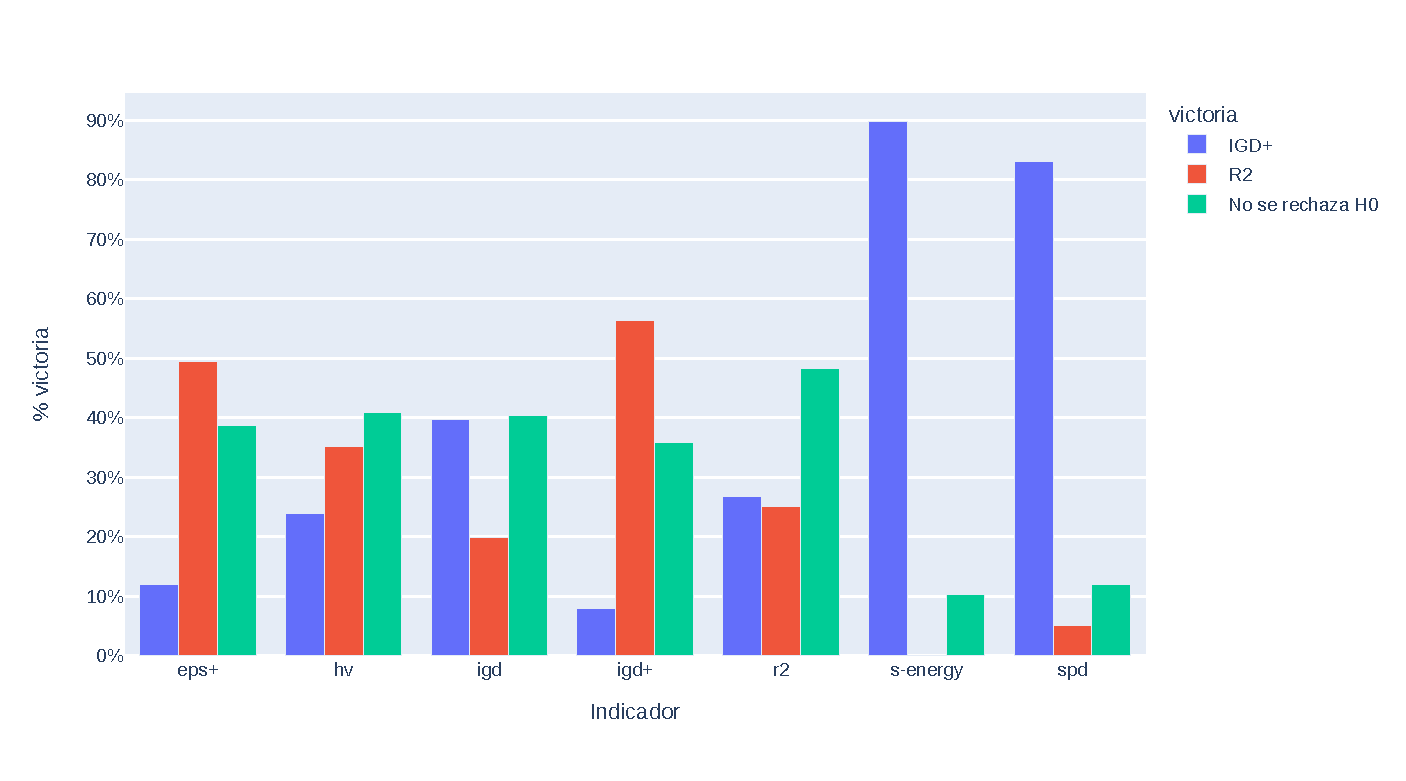
\includegraphics[width=\textwidth]{Figuras/R2_vs_IGDp_nobj6.pdf}
\caption[IGD+ vs R2 6 objetivos]{Porcentaje de victorias de diferentes indicadores de convergencia en la esclarización de Tchebycheff para 6 objetivos.}
\label{fig:R2_vs_IGDp_6}
\end{figure}

\begin{figure} [H]
    \centering
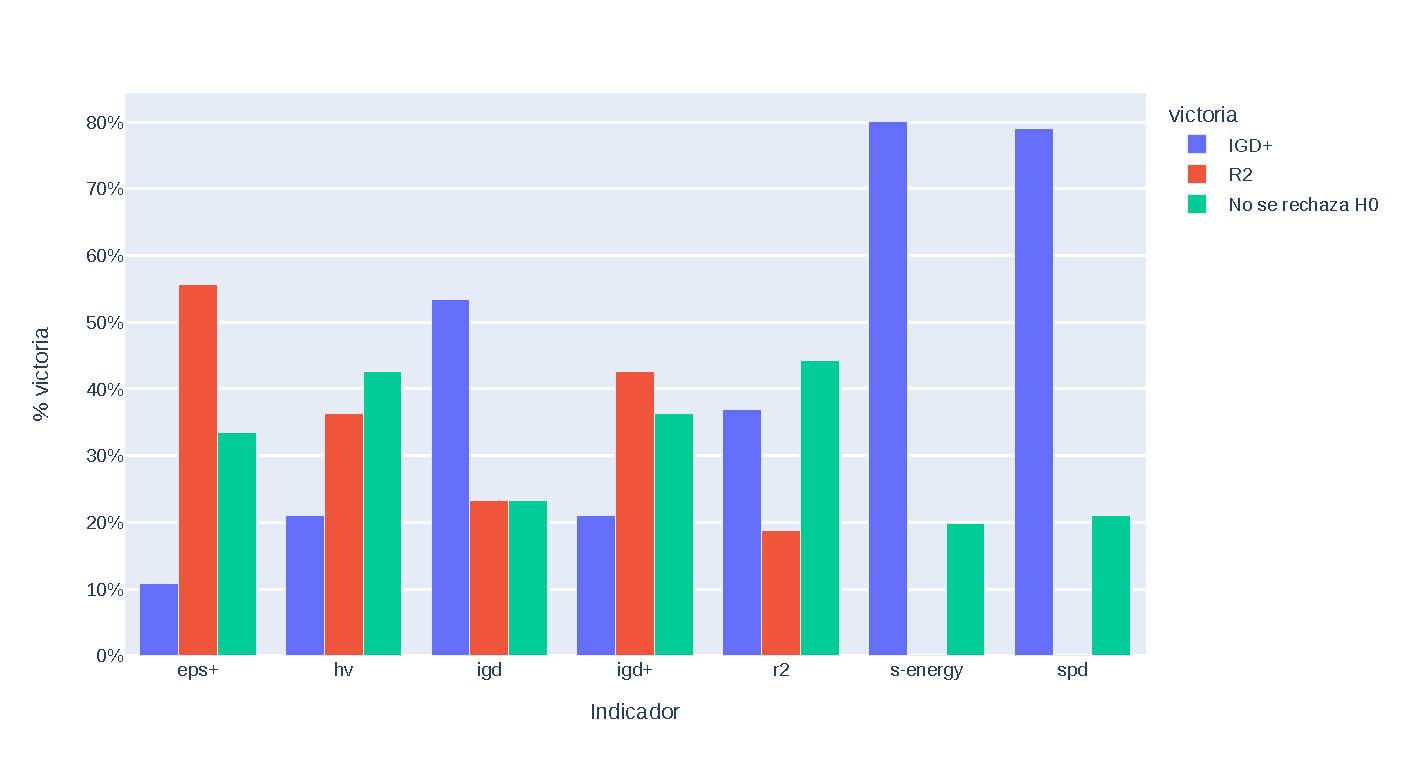
\includegraphics[width=\textwidth]{Figuras/R2_vs_IGDp_nobj7.pdf}
\caption[IGD+ vs R2 7 objetivos]{Porcentaje de victorias de diferentes indicadores de convergencia en la esclarización de Tchebycheff para 7 objetivos.}
\label{fig:R2_vs_IGDp_7}
\end{figure}

De las Figuras \ref{fig:R2_vs_IGDp_2}, \ref{fig:R2_vs_IGDp_3}, \ref{fig:R2_vs_IGDp_4}, \ref{fig:R2_vs_IGDp_5}, \ref{fig:R2_vs_IGDp_6} y \ref{fig:R2_vs_IGDp_7}  podemos ver con una comparación directa que los algoritmos de IGD+ tienden a tener mejor desempeño que los de IGD. Teniendo excepciones para 5 objetivos, como podemos ver en la Figura \ref{fig:R2_vs_IGDp_5}, en los indicadores IGD+ y R2, donde el algoritmo de R2 tiene mejor desempeño en promedio. No podemos concluir porqué es que esto ocurre sólo para este caso, pero es un buen problema para trabajo futuro.

Un resultado interesante de estas últimas gráficas es que, aunque R2 no es tan sensible a cambiar su desempeño conforme se cambia $w_0$, su desempeño se vuelve mejor conforme subimos las dimensiones. Habiendo casos donde aunque no haya mucha diferencia entre los diferentes pesos para R2, tiene mejor desempeño que IGD+. En 2 y 3 dimensiones los resultados están muy dominados por IGD+. 

También hacemos las comparaciones análogas a las hechas para diferente número de objetivos, pero con el tipo del indicador y presentamos los resultados en la Figura \ref{fig:R2_IGDp_cat}.


\begin{figure}[H]
    \centering
    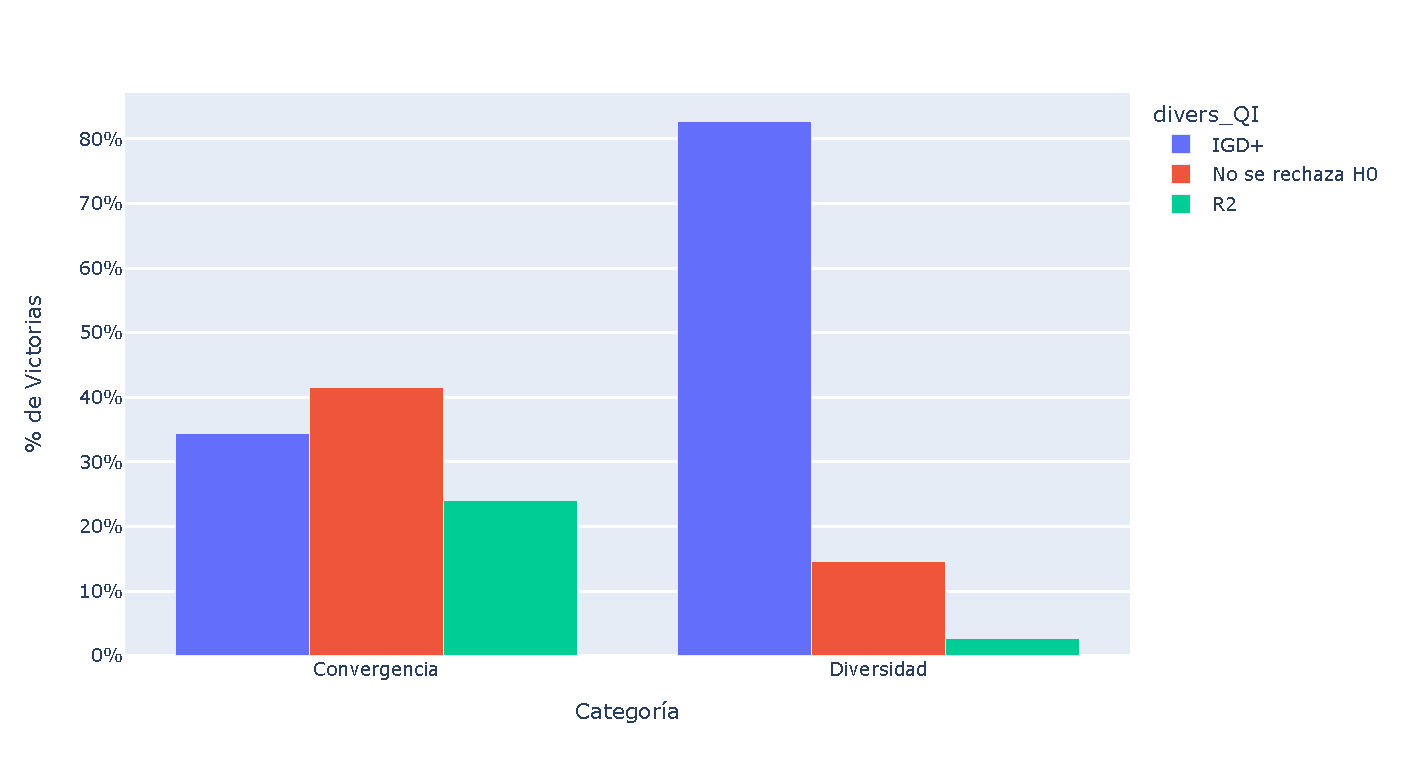
\includegraphics[width=\textwidth]{Figuras/R2_vs_IGDp_por_tipo_ind.pdf}
    \caption[R2 vs IGD+, victorias por indicador.]{Comparaciones de victorias de cada algoritmo para cada $w_0$ tomando en cuenta el tipo de indicador que se está optimizando.}
    \label{fig:R2_IGDp_cat}
\end{figure}


Vemos que IGD+ gana más veces que R2 sin embargo para los indicadores de convergencia hay más casos donde no se puede concluir que no se rechaza la hipótesis nula de una distribución simétrica alrededor del 0. En los indicadores de diversidad existe mucha preferencia por los de IGD+. Lo que nos podría hablar de preferir este tipo de algoritmos sobte los de R2 cuando se realice este análisis. 


Finalmente, en la Figura \ref{fig:R2_IGDp}, presentamos el análisis con mayor agrupación en el que comparamos directamente los algoritmos de R2 e IGD+ a través de todos los pesos, pareando las diferentes combinaciones de pesos, pero sin hacer ninguna otra división. 


\begin{figure}[H]
    \centering
    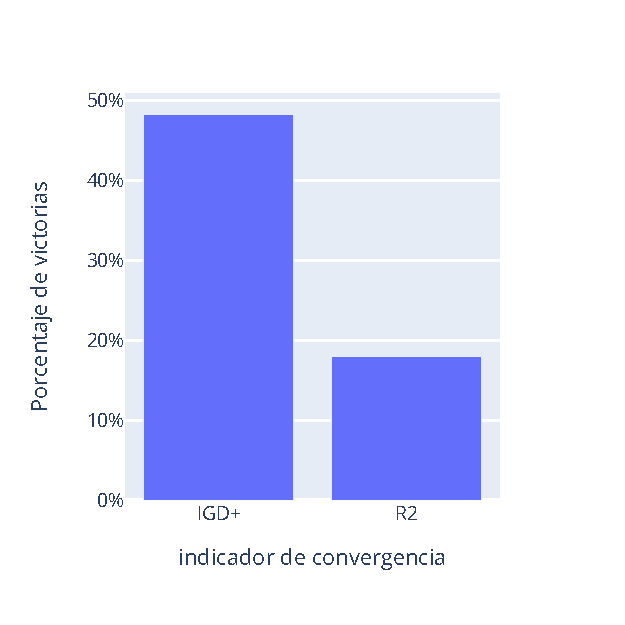
\includegraphics[scale=.7]{Figuras/R2_vs_IGDp.pdf}
    \caption[Victorias por algoritmo]{Victorias de cada algoritmo. El restante del $100\%$ son en las que no se rechazó la hipótesis nula.}
    \label{fig:R2_IGDp}
\end{figure}


Una vez más vemos que IGD+ tiene un mejor desempeño que R2 en el agregado, sin embargo, el detalle es importante para escoger que usar en cada problema. 

Habiendo presentado una breve discusión de los resultados, en el capítulo siguiente daremos ideas de cómo mejorar y hacer más formales estos resultados. 



